\chapter{Exploring Bifurcations between Phenotypes}
\label{chapter:exploring}
\begin{music}
    \parindent10mm \instrumentnumber{1} \setstaffs1{1} 
    \generalmeter{\meterfrac44} \generalsignature{-1}
    \startextract
            \notes \ql k \Dqbl mk \ql o \ql m \en
        \bar \zw{q*}
    \zendextract
\end{music}
\epigraph{\textit{who knows what might happen to those who are consumed by greed}}{Requiem of Spirit --- Ocarina of Time}
\section{Preface}
\subsection{Problem Statement \& Context}
The studies in chapters \ref{chapter:double-exclusive}--\ref{chapter:inference} were carried out under the assumption that the underlying microscopic mechanisms that give rise to different phenotypes of an organism are known, and therefore can be modelled with differential equations that have interpretable parameters $\theta$. In section \ref{section:phenotype-inference} we outlined some popular machine learning approaches that can be used in settings where the underlying mechanism is partially or completely unknown. This chapter presents a study in immunology. While detailed models of the immune system exist \cite{Eftimie2016MathematicalDirections}, in the advent of high-throughput biology new mechanisms and exceptions are continuously being discovered \cite{Varade2020HumanChallenges}. This is done by identifying immune cell populations, their function and mechanism of action from tissue and blood samples taken from an organism in homeostasis. \emph{Immunophenotyping} methods use antibodies to identify cells based on the types of antigens or markers on their surface. As we shall see, such datasets are typically high-dimensional data clouds that can be reduced with the help of \emph{universal function approximators} and clustered to identify different immune cell phenotypes. Such high-dimensional data clouds also appear in Chapter \ref{chapter:inference} when optimal parameters $\theta$ reveal clusters of topologically or geometrically equivalent models.

In this chapter we argue the importance of interactive tools that allow immunologists to navigate high-dimensional data clouds from heterogeneous experimental setups. Such tools enable crowd-sourced consensus phenotyping of cell populations, discovery of rare populations and iterative refinement of a model of the immune system. An interactive tool \emph{FlowAtlas.jl} (\texttt{github.com/gszep/FlowAtlas.jl}) is presented in an adaptation of a manuscript being prepared at the time of writing the thesis. We conclude this chapter with a vision of how approaches in chapters \ref{chapter:inference} and \ref{chapter:exploring} can be combined to realise a high-throughput \emph{design--learn} pipeline.

\subsection{Contributions}
The following sections are an adaptation by \textbf{Grisha Szep} which deliberately omits details in the biology and experimental design in favour of thesis narrative, and will differ from the submitted manuscript. \textbf{Grisha Szep} is co-first author with \textbf{Valerie Coppard} and \textbf{Sarah Howlett}. \textbf{Joanne Jones}, \textbf{Daniel Rainbow}, \textbf{Sarah Howlett} and \textbf{Lorna Jarvis} conceived and designed the study. \textbf{Sarah Howlett}, helped by \textbf{Daniel Rainbow} and \textbf{Lorna Jarvis} acquired and processed donor tissue samples. Furthermore \textbf{Ondrej Suchanek}, \textbf{Edward J. Needham}, \textbf{Hani S. Mousa}, \textbf{David Menon}, \textbf{Krishna Mahbubani} and \textbf{Kourosh Saeb-Parsy} helped acquire and process the tissues. \textbf{Valerie Coppard} designed the flow cytometry panels, performed the experiments and exported figures from FlowAtlas and FlowJo. \textbf{Grisha Szep} conceived and implemented the computational pipeline and interactive software. All authors analysed, interpreted data and tested software.

\fakesection{Abstract}

\noindent\makebox[\linewidth]{\rule{\linewidth}{4pt}}
\begin{center}
    \Large \bfseries FlowAtlas.jl: an interactive tool bridging\\ FlowJo with computational tools in Julia
\end{center}
\noindent\makebox[\linewidth]{\rule{\linewidth}{1pt}}\\
{ \bfseries
    Valerie Coppard$^{1,3,+}$, Grisha Szep$^{2,+}$, Sarah K. Howlett$^{3,+}$, Lorna B. Jarvis$^{3}$, Daniel B. Rainbow$^{3}$, Zoya Georgieva$^{3}$, Suchanek O$^{4}$, Edward J. Needham$^{3}$, Hani S. Mousa$^{3}$, David K. Menon$^{5}$, Krishna T. Mahbubani$^{6}$, Kourosh Saeb-Parsy$^{6}$, and Joanne L. Jones$^{3}$
}\\{\footnotesize
$^{1}$Microsoft Research Cambridge, Station B, Cambridge\\
$^{2}$King's College London, Randall Centre for Cell \& Molecular Biophysics, London\\
$^{3}$University of Cambridge, Department of Clinical Neurosciences, Cambridge\\
$^{4}$University of Cambridge, Department of Medicine, Cambridge\\
$^{5}$Department of Anaesthesia, University of Cambridge, Cambridge\\
$^{6}$Department of Surgery, University of Cambridge, Cambridge\\
$^{+}$Co-first authors 
}\\
\begin{center}
\begin{minipage}{10cm}
    \noindent As the dimensionality, throughput, and complexity of cytometry data increases, so does the demand for user-friendly, interactive analysis tools that leverage high-performance machine learning frameworks. Here we introduce \emph{FlowAtlas.jl}: an interactive web application that bridges the familiar user-friendly environment of FlowJo and computational tools in Julia developed by the scientific machine learning community. We demonstrate the capabilities of FlowAtlas using a novel human multi-tissue, multi-donor immune cell dataset, highlighting key immunological findings.
\end{minipage}
\end{center}
\pagebreak

\section{Introduction}
Rapid advancements in flow and mass cytometry have brought about a new era of high-dimensional cell phenotyping \cite{Cheung2021CurrentSoftware}. However, new algorithms and computational methods for dealing with high-dimensional data are typically not accompanied by user-friendly, flexible and interactive analysis tools. The wider biomedical research community relies on intuitive and transparent analysis for reaching consensus on discoveries. The uptake of currently available computational tools by biologists remains low, likely due to the lack of inter-operability with familiar platforms such as FlowJo or FCSExpress \cite{Cheung2021CurrentSoftware} and high entry requirements for computational literacy. Here we introduce FlowAtlas -- our effort to address the following issues:

\begin{itemize}
    \item Comparing insights from immunophenotyped datasets from heterogeneous experimental designs is difficult
    \item Navigating high-dimensional data in well-established tools like FlowJo or FCSExpress is difficult
    \item Limited computational resources require down-sampling data that may contain rare populations
    \item Pipelines built in scripting languages like R or Python have limited inter-operability with FlowJo
\end{itemize}

\begin{Figure}
    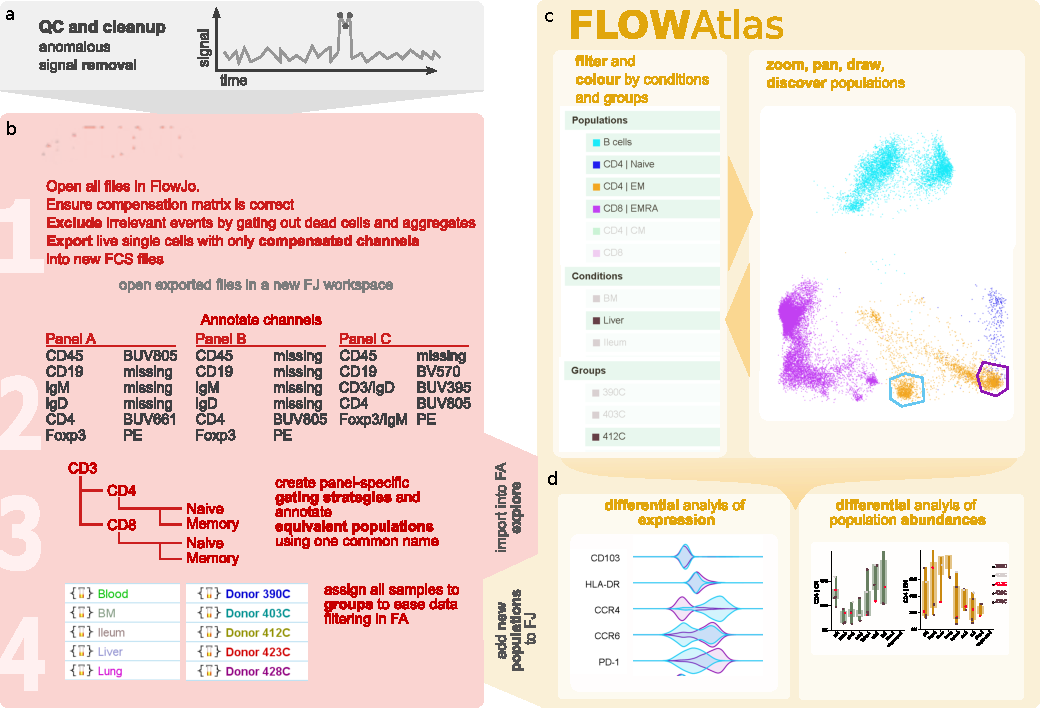
\includegraphics[width=\linewidth]{flow-atlas}
    \caption{Overview of FlowAtlas workflow with FlowJo. Left: Processing in FlowJo includes: signal compensation and filtering, annotation of channels, sample groups and cell populations with gating strategies. Processing in FlowJo is limited by two dimensional scatter plots. Right: FlowAtlas enables interactive navigation of high-dimensional embedding. Cells can be filtered and coloured by any property on \emph{Annotations} tab. Regions of interest can be drawn in the embedding to generate violin plots in the \emph{Expression} tab. Box plots are generated from group annotations and filter selection in the \emph{Frequency} tab. New phenotypes and activation states identified in FlowAtlas can be validated in FlowJo}
    \label{fig:flow-atlas}
\end{Figure}

We showcase the capabilities of FlowAtlas using a novel human flow cytometry dataset consisting of immune cells extracted from the tissues of five deceased organ donors. Immunophenotyping was performed using three slightly different antibody panels (see Tables \ref{table:donors}--\ref{table:panels} for donor metadata and panel information) representing heterogeneity in experimental design that is typical across multiple datasets. FlowAtlas was designed for use in an iterative discovery loop with FlowJo, where traditional FlowJo gating strategies provide initial annotation of main cell populations, conditions, and sample grouping to guide the discovery of new sub-populations. With the help of a high-performance visualisation library \texttt{GigaSOM.jl} \cite{Kratochvil2018RapidEmbedSOM}, we can perform a two dimensional embedding of high-dimensional datasets without down-sampling. The scatter visualisation methods from \texttt{GigaSOM.jl} were exposed to a browser front-end with interactive library OpenLayers \cite{MetaCarta2006OpenLayers}. This enabled the visual exploration and profiling of hundreds of millions of cells. By imputing missing values before dimensionality reduction, using random sampling with replacement, datasets acquired using non-identical antibody panels can be integrated and analysed together. To remove any biases induced by algorithms or data processing, the imputed values are neither visualised nor included in any downstream analysis.

\section{Proposed Method}

\subsection{Pre-processing}
When using a flow cytometer, acquisition anomalies can result from sudden flow rate or signal acquisition instability and induce undesired spearing in population distributions \cite{Lee2001HydrodynamicCytometer}. The proposed pipeline filters these anomalies using an existing method called FlowAI \cite{GianniMonaco2017FlowAI}. Filtered files are then imported into FlowJo for data pre-processing, which includes quality control of compensation matrices and gating of live lymphocytes using forward, side scatter and zombie dye channels. The resulting live lymphocytes data are then exported as new files, reducing the file size by approximately 40\%. This substantially shortens the time to carry out the computationally expensive embedding algorithm. FlowJo is then used to annotate channels and resolve discrepancies between channel names that were defined at acquisition time from different panels. In our dataset, for example, some samples only had the signal from FoxP3 while others had both FoxP3 and IgM markers in a single channel. By renaming FoxP3 to FoxP3-IgM in the relevant samples in FlowJo we can analyse both sample sets together in FlowAtlas. Missing channels between datasets are imputed only for the purposes of calculating the embedding.

\subsection{Annotation in FlowJo}
Hierarchical gating strategies (Figure \ref{fig:gating}) are used to annotate known populations of interest. These strategies can differ between samples and panels as long as gates that define the same phenotype are given the same name. Cells that fall outside of the gating strategy are annotated as \textit{unlabelled} in FlowAtlas and can still be explored. The filters that can be used to navigate and colour-code the embedding are defined by the sample group names in FlowJo. In this dataset, each sample is allocated to two groups: one telling us which tissues the sample came from, the other identifying the donor. By default, groups are interpreted as different \textit{conditions} of a sample, unless the group name contains numbers, in which case the group is interpreted as a \textit{batch}. The user can rename and rearrange groups in FlowAtlas to control this interpretation. In our dataset the \textit{conditions} are different tissues and \textit{batches} are different donors.
\begin{Figure}
    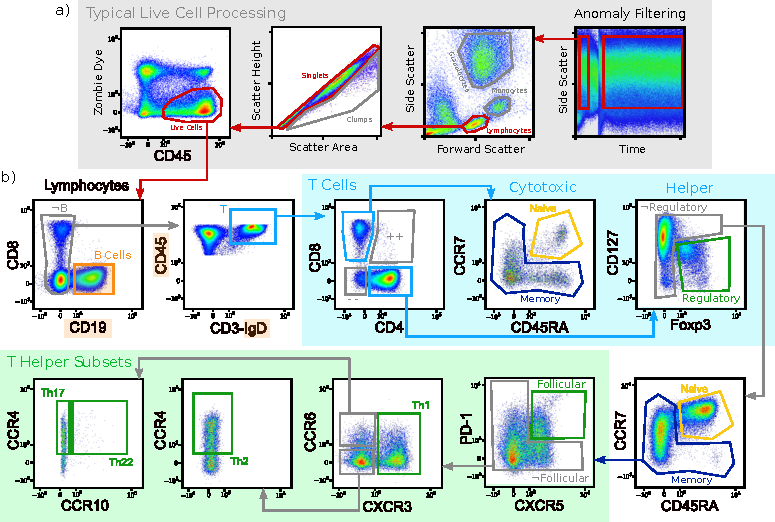
\includegraphics[width=\linewidth]{gating}
    \caption{Gating strategy for a given condition and batch. \textbf{a} A typical strategy for extracting live singlet lymphocytes, reducing the dataset size by 40\%. \textbf{b} Immunophenotyping strategy for identifying T-helper subsets. Any or all of the following channels (highlighted in orange) may be missing due to heterogeneous panel design: CD19, IgD and CD45}
    \label{fig:gating}
\end{Figure}

\subsection{Exploration in FlowAtlas.jl}
The information from the FlowJo workspace is loaded and parsed by FlowAtlas. Individual files are merged into one table and missing values are imputed for the purpose of the embedding. The embedding mapping is cached in a file named with a \texttt{.som} extension. The same mapping can be used for different datasets as long as the channel names and the total number of channels match. To re-calculate the mapping, one simply deletes the cache file. Sharing the cache file together with the FlowJo workspace and FCS files allows colleagues to work on the same embedding to verify findings in a reproducible manner. 

The graphical user interface (Figure \ref{fig:flow-atlas}) has a map of the two dimensional embedding that was obtained by dimensionality reduction with EmbedSOM \cite{Kratochvil2020GigaSOM.jl:Datasets}. The map can be zoomed and panned and is rendered efficiently using OpenLayers \cite{MetaCarta2006OpenLayers}. The left-hand panel menu was designed with D3.js \cite{Bostock2011D3.js} and has four tabs: \textit{Annotations}, \textit{Expression} and \textit{Frequency}. The \textit{Annotations} tab allows the user to filter and colour the embedding by marker expression, population, condition and batch information imported from FlowJo. The conditions and batches can also be redefined here. The \textit{Expression} tab has a polygon draw tool that enables gating populations directly in the embedding filtered by settings in the \textit{Annotations} tab. The gates are then used to produce violin plots that reveal fluorescence distributions across all markers. By clicking the violins it is possible to re-colour the gates to perform a differential expression analysis. The \textit{Frequency} tab generates box plots showing relative abundance of selected populations and conditions relative to any set of parent populations. The parental population, the \textit{conditions} axis and \textit{batch} marker colours are defined by settings in the \textit{Annotations} tab. Unique sub-populations identified in FlowAtlas can then be validated in FlowJo. This iterative discovery loop facilitates the identification of rare phentypes that may otherwise be missed by due to down-sampling or under-fitting in unsupervised clustering approaches.

\section{Results}
It has become common-place in single cell analysis publications to include a two dimensional embedding that reveals different cell phenotypes as clusters in the scatter plot \cite{Liu2020RecentData}. While providing a global overview of the dataset, such static images are difficult to interrogate for batch variance and possible subset structures that may imply there are unlabelled phenotypes present that were not captured by the gating strategy (Figure \ref{fig:gating}). FlowAtlas provides an interactive interface for filtering, colouring and zooming into an embedding for efficient phenotype discovery. By filtering and colouring by batch, it is possible to readily identify batch effects and subsets that are conserved across batches (Figure \ref{fig:treg-batches}). 
\begin{Figure}
    \includegraphics[width=\linewidth]{treg-batches}
    \caption{Detecting batch variance within the regulatory helper phenotype. \textbf{a} Regulatory to helper ratio by tissue aggregated over batches reveals enrichment in lymph nodes and blood. \textbf{b} Self-organised map embedding of all regulatory cells coloured by Helios expression. A region of high Helios expression can be identified and zoomed, in searched for subsets. \textbf{c} Embedding coloured and filtered by different batches to identify conserved subsets. Fluorescence distributions reveal missing channels and batch effects.}
    \label{fig:treg-batches}
\end{Figure}
Once the subsets conserved across batches have been identified they can be gated directly in the embedding (Figure \ref{fig:treg-discovery}). Filtering the embedding by tissue will give us an initial estimate for the relative abundance of the newly identified subsets. The fluorescence distributions for each gate will guide additions to the gating strategy in FlowJo.
\begin{Figure}
    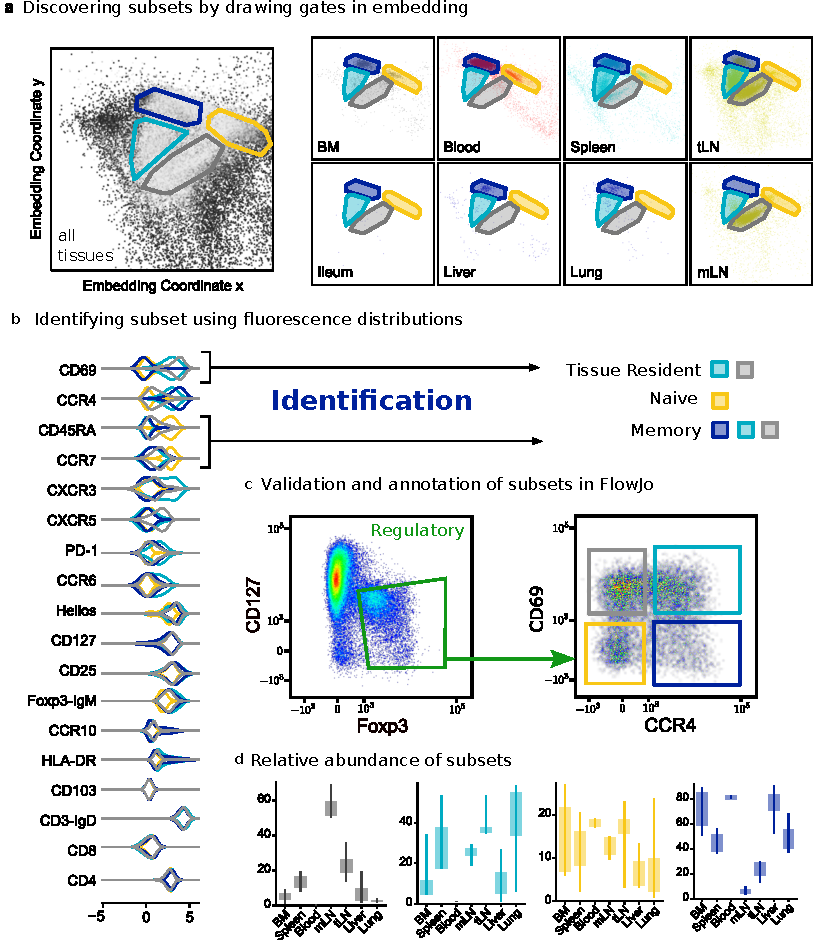
\includegraphics[width=0.9\linewidth]{treg-discovery}
    \caption{Identification of regulatory subsets. \textbf{a} Gating in the embedding and filtering by tissue reveals certain populations are not present in blood. \textbf{b} Fluorescence distributions reveal tissue resident, naive and memory phenotypes. \textbf{c} Channels that distinguish subsets can be gated in FlowJo for validation and annotation. \textbf{d} New annotations can be used to calculate relative abundance, verifying the absence of memory subsets in blood and enrichment in tissues}
    \label{fig:treg-discovery}
\end{Figure}

\subsection{Regulatory Helper Subsets}
Regulatory T helper cells suppress immune response and thereby maintain homeostasis and self-tolerance. It has been shown that regulatory helpers are able to inhibit T cell proliferation and cytokine production and play a critical role in preventing autoimmunity \cite{Kondelkova2010RegulatoryDisorders}.

In our dataset, regulatory helpers were enriched in mesenteric lymph nodes (mLN) accounting for more than 20\% of all helper cells across all donors (Figure \ref{fig:treg-batches}a). Colouring the embedding of regulatory helper cells by the expression of the Ikaros family transcription factor Helios (Figure \ref{fig:treg-batches}b) revealed Helios$^+$ and Helios$^-$ subsets as expected \cite{Thornton2019Helios:Clouds,Himmel2013Helios+Humans}. While inter-batch variability existed, the relative positions of four clusters within the Helios$^+$ subset was conserved (Figure \ref{fig:treg-batches}c). Differential expression in violin plots revealed variation due panel design: higher CD4 fluorescence intensity for one batch due to use of a different dye (Table \ref{table:panels}).

Four subsets within Helios$^+$ could be identified and gated to obtain fluorescence distributions (Figure \ref{fig:treg-discovery}b) which revealed that CD69, CCR4, CD45RA and CCR7 and explain the majority of variability between clusters. We identify one naive regulatory helper phenotype (CD45RA$^+$, CCR7$^+$) and three populations showing characteristics of the memory phenotype (CD45RA$^-$, CCR7$^-$). The memory subsets can be further subdivided in a CCR4,CD69 quadrant and verified on FlowJo (Figure \ref{fig:treg-discovery}c). Two subsets were found to express CD69$^+$, a marker of tissue residency that promotes retention through sequestration of the \emph{sphingosine-1-phosphate} receptor \emph{S1P1} required for their egress \cite{Shiow2006CD69Organs,Kumar2017HumanSites,Sathaliyawala2013DistributionSubsets}. Dividing the embedding by tissue revealed tissue-specific enrichment patterns with blood lacking the CD69$^+$ subsets consistent with their tissue residency phenotype (Figure \ref{fig:treg-discovery}d). Lung and liver contained a high proportion of regulatory helpers expressing the chemokine receptor CCR4. CCR4 has been reported to play an important role in T cell trafficking to the lung \cite{Mikhak2013LungCCR4} and in the infiltration of regulatory helpers into tumours \cite{Bromley2008OrchestratingTraffic}. 

Similar to how we've shown for regulatory T helper cells here, this iterative discovery loop can be performed for any other population of interest. We now proceed to a second example in which we explore Th1 helper cells.

\subsection{Th1 Helper Subsets}
Th1 helper cells prime the immune response against intracellular microorganisms including, viruses, intracellular bacteria, and some intracellular parasites. This is done by the secretion of cytokines, small protein mediators that activate and recruit macrophages and cytotoxic T cells to target cells to a site of infection.

\begin{Figure}
    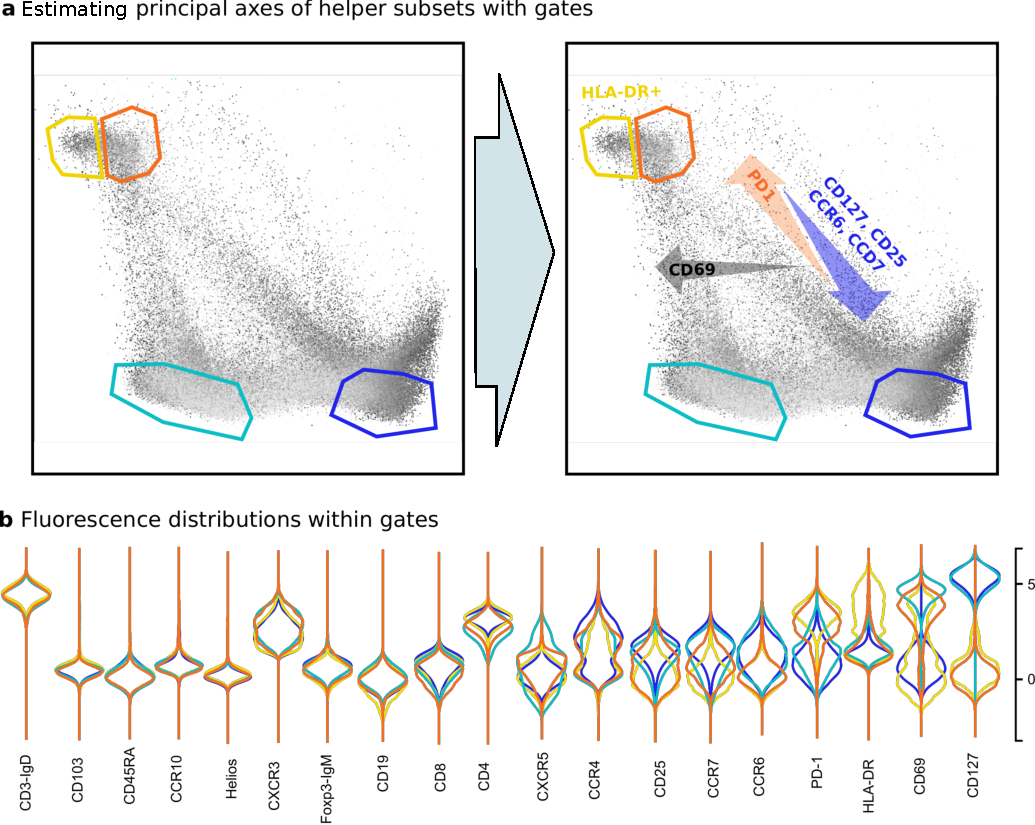
\includegraphics[width=0.9\linewidth]{th1}
    \caption{\textbf{a} Estimating the local principal axes in the embedding for Th1 helper subsets. \textbf{b} Fluorescence distributions within gates reveal correlations}
    \label{fig:th1}
\end{Figure}

An exploratory analysis of Th1 helper subsets reveals that the population distribution is supported on a simplex, whose principal axes can be constructed from correlations between fluorescence channels (Figure \ref{fig:th1}). Cells characterised by the co-expression of CD69 and CD127 are lacking blood, consistent with tissue residency.

\section{Discussion}
\label{exploring:discussion}
In conclusion, FlowAtlas brings a new iterative analysis concept to biomedical scientists by linking the familiar FlowJo workflow with a high-performance machine learning framework in a fully graphical, interactive environment. FlowAtlas allows rapid computation of embedding of millions of high-dimensional events on an average laptop without the need for down-sampling. The resulting embedding is highly interactive, offering zooming to explore deeper cluster structures, colouring and filtering of embedded events by custom conditions, the generation frequency statistics and the drawing of gates directly in the embedding for comparative analysis of marker expression. Moreover, state-of-the-art missing data handling methods enable concomitant cross-study analysis of datasets with non-identical panel designs or marker numbers. Findings can be immediately validated in FlowJo in an iterative discovery loop with FlowAtlas simplifying the identification and validation of rare or novel cell populations, which are more likely to be detected in the absence of down-sampling. FlowAtlas aims to strengthen the open-source collaborations between researchers using flow cytometry and the rapidly growing scientific machine learning community in Julia programming language.

A significant amount of time was spent adjusting the gating strategy which formed the initial annotations of different immune cell phenotypes. One point of disagreement was how sensitive biological findings and conclusions were to adjustments in the gating strategy. Sensitivity methods would resolve such issues. Furthermore, there is often disagreement between experts on how gates should be placed and what the appropriate anomaly filtering, compensation and non-linear transformation settings should be. Domain knowledge often leads immunologists to ask specific questions and annotate populations at the tails of distributions rather than their density centres. Clustering approaches, that may provide us with gating strategies automatically, typically lack the flexibility to define such populations. The immunologist wants the ability to intervene with their own annotations at any given stage of data processing.

The emerging picture suggests that building a crowd-sourced differentiable gating annotation tool would be valuable to the flow cytometry community. Community consensus annotations of large datasets are used by consumer internet businesses like Google and Microsoft on a regular basis to provide training data for their machine learning algorithms \cite{Vaughan2018MakingResearch}. Differentiability enables the application of sensitivity and optimisation methods which would be reveal the most robust annotations with highest consensus, and perhaps more importantly, reveal disagreement and ambiguity in biological findings, guiding the design of future experiments. The resolution of disagreement can be further incentivised with micro-transactions, thus potentially requiring the use of Web3 technology. The term \emph{decentralised science} \cite{Hamburg2021CallMovement} has already been coined but yet to have an established movement behind it.

The dimensionality reduction method \emph{EmbedSOM} \cite{Kratochvil2018RapidEmbedSOM} was not designed with interaction in mind. In principle it would be possible to provide continuous updates to the two dimensional embedding parameters based on the zoom and pan parameters of the field of view. Reduction methods already exist that leverage hyperbolic embeddings \cite{Peng2021HyperbolicSurvey} which allow more information from higher dimensions to be packed into a lower dimensional non-euclidean space. Combining these methods with interactive elements, perhaps even using virtual reality \cite{Reski2020OpenTechnology}, may enable researchers to gain a more intuitive grasp of high dimensional datasets by interactively zooming between global and local structures.